\section{Experiments}
\label{sec:experiments}

In this section we describe experiments based on our testing framework. 

%%%%%

\begin{figure}
\begin{center}
\begin{tabular}{lccc}
Category            & Arity & Stateful? & Heterogeneous? \\ \hline
Synchronous channel & 2     & N         & Y \\
Filter channel      & 2     & N         & Y \\
Men and women        & 2     & N         & Y \\
Exchanger           & 2     & N         & N \\
Two families        & 2     & Y         & Y \\
One family          & 2     & Y         & N \\
ABC                 & 3     & N         & Y \\
Barrier             & $n$   & N         & N \\
Timeout channel     & 2, 1  & N         & Y \\
Timeout exchanger   & 2, 1  & N         & N \\
Closeable channel   & 2, 1  & Y         & Y \\
Terminating queue   & 1, $n$ & Y        & N  
\end{tabular}
\end{center}
\caption{Example interfaces of synchronisation objects.  \label{fig:examples}}
\end{figure}

% Channel with counter & 2    & Y         & Y \\
% ABC with counter    & 3     & Y         & Y \\
% Barrier with counter & $n$  & Y         & N \\   
% Add combining barrier?    

%%%%%

We consider synchronisation objects implementing a number of interfaces,
summarised in Figure~\ref{fig:examples}.  Most of the interfaces were
described in earlier sections (namely synchronous channel, filter channel,
exchanger, barrier, timeout channel, closable channel, terminating queue).
The \emph{men and women} problem involves two families of threads, known as
men and women: each thread wants to pair off with a thread of the other type;
each passes in its own identity, and expects to receive back the identity of
the thread with which it has paired.  In the \emph{two families} problem,
there are two families of threads, with $n$~threads of each family; each
thread calls an operation~$n$ times, and each invocation should synchronise
with a thread of the opposite family, a different thread each time.  In the
\emph{one family} problem, there are $n$~threads, each of which calls an
operation $n-1$~times, and each time should synchronise with a different
thread.  The \emph{ABC} problem can be thought of as a ternary version of the
men and women problem: there are three types of threads, A, B and C; each
synchronisation involves one thread of each type.  Finally, the \emph{timeout
  exchanger} is a timed version of the exchanger: if a thread fails to
exchange data with another thread, it can timeout and return an appropriate
result.

%% For each interface, we have implemented a tester, using the appropriate
%% algorithm from earlier sections.  When considering synchronisation
%% linearisation, in most cases, the invocations performed by threads had to be
%% chosen so that every invocation will synchronise, so as to avoid deadlocks.
%% For example, for the synchronous channel tester, half the threads perform
%% sends, and half perform receives; in the exchanger tester, each thread ran a
%% single invocation (or else a slow thread could get stuck).

%% For synchronisation objects involving data, the data values were chosen
%% randomly from a reasonably large range (e.g.~$\range{0}{100}$); this makes it
%% easier for the algorithm to identify matchings, and also makes it easier for
%% the user to understand any incorrect histories that are detected.  The
%% implementations are data independent~\cite{???}: they store and return the
%% data, but otherwise their operation does not depend on the data values used;
%% this means that the data values used do not affect the occurrences of bugs.

For each interface, we have implemented a tester, using the appropriate
algorithm from earlier sections, and have produced a correct implementation.
For most interfaces, we also implemented one or more faulty versions that fail
to achieve either synchronisation linearisation or progressibility.  The
faulty versions mostly have realistic mistakes, mistakes that we believe
programmers could make.

We describe various experiments below: some concern the time required to find
bugs; and some concern the throughput for correct versions.
%
The experiments were performed on an eight-core machine (two 2.40GHz Intel(R)
Xeon(R) E5620 CPUs, with 12GB of RAM).

In each experiment below, we performed \emph{observations}, by running a
tester and recording the time taken.  Each observation aims to reflect a
typical use case.  In each experiment we performed multiple observations; we
give the average running time and a 95\%-confidence interval.  Each
observation was run as a separate operating system process, to ensure
independence.  The number of observations is chosen so as to obtain a
reasonably small confidential interval, but avoiding excessively long
experiments.

%%%%%%%%%%%%%%%%%%%%%%%%%%%%%%%%%%%%%%%%%%%%%%%%%%%%%%%

%\subsection{Tuning}

Most of the testers have a number of parameters.  The parameters that are
likely to have the biggest effect on the likelihood of finding bugs are
%
\begin{itemize}
\item the number of threads to run;
\item the number of invocations to be performed by each thread in a run.
\end{itemize}
%
We ran experiments on two testers, using incorrect implementations of a
synchronous channel and the ABC problem, to investigate how the time taken to
find an error is affected by these two parameters.  Each observation used
particular values for these parameters, performed repeated runs until an error
was found, and recorded the time taken.  (Note that the two testers assume
that the number of threads is divisible by two or three, respectively; and we
believe that the error in the ABC case requires more than three threads.)  For
each choice of parameters, 200 observations were performed.
Figure~\ref{fig:tuning} gives results, displaying average times and
95\%-confidence intervals.

%%%%%%%%%%%%

\begin{figure}
\begin{minipage}{0.5\textwidth}
%% \documentclass[a4paper]{article}
%% \usepackage{pgfplots}
%% \pgfplotsset{compat=1.16}
%% \begin{document}

\begin{tikzpicture}
\begin{semilogxaxis}[
%  title = Experiment on the time taken to find a bug,
  ylabel = Time (ms),
  xlabel = Invocations per thread,
  % ymax = 4,
  log basis x=2,
  scaled ticks = false,
  legend pos = north west,
  height = 0.4\textheight,
  width = 0.90\textwidth
]
\addplot+[error bars/.cd, y dir=both,y explicit] coordinates {
  (2,83.08509326000001) +- (0,1.2354531362387784)
  (4,74.88299255) +- (0,1.3112835057583532)
  (8,79.067596255) +- (0,1.9395745438227188)
  (16,80.47892682999999) +- (0,2.0364739691984073)
  (32,80.797998155) +- (0,1.8239378697908442)
};
\addlegendentry{$p = 2$}
\addplot+[error bars/.cd, y dir=both,y explicit] coordinates {
  (2,87.516821685) +- (0,1.4792666407834463)
  (4,81.817856485) +- (0,1.651014381813079)
  (8,84.73854852) +- (0,2.6680012145096885)
  (16,89.37923438) +- (0,2.1757320329956484)
  (32,95.14338612) +- (0,2.828884694709013)
};
\addlegendentry{$p = 4$}
\addplot+[error bars/.cd, y dir=both,y explicit] coordinates {
  (2,94.39215556) +- (0,2.1871718235223345)
  (4,89.20503961) +- (0,1.423227793928453)
  (8,97.728336265) +- (0,2.663437124298785)
  (16,106.08867011) +- (0,3.660762475944014)
  (32,117.08226379000001) +- (0,3.54637813404394)
};
\addlegendentry{$p = 8$}
\addplot+[error bars/.cd, y dir=both,y explicit] coordinates {
  (2,99.684097325) +- (0,2.1639888413012356)
  (4,101.14500844499999) +- (0,1.1203456199995476)
  (8,115.256713) +- (0,3.5984690955172924)
  (16,122.60207184000001) +- (0,1.190600621017305)
};
\addlegendentry{$p = 16$}
\end{semilogxaxis}
\end{tikzpicture}

% --samples 200 --tester ChanTester --maxItersPerRun 256
%\end{document}

\end{minipage}
%
\begin{minipage}{0.5\textwidth}
%% \documentclass[a4paper]{article}
%% \usepackage{pgfplots}
%% \pgfplotsset{compat=1.16}
%% \begin{document}

\begin{tikzpicture}
\begin{semilogxaxis}[
  % title = Experiment on the time taken to find a bug,
  ylabel = Time (ms),
  xlabel = Invocations per thread,
  % ymax = 4,
  log basis x=2,
  scaled ticks = false,
  legend pos = north west,
  height = 0.4\textheight,
  width = 0.9\textwidth
]
\addplot+[error bars/.cd, y dir=both,y explicit] coordinates {
  (2,5871.77268287) +- (0,1241.652477706246)
  (4,744.931896425) +- (0,100.39702970192621)
  (8,932.286987545) +- (0,70.12118940035633)
  (16,1720.175756855) +- (0,299.7126481558856)
  (32,7054.778178755) +- (0,1090.8275119367097)
};
\addlegendentry{$p = 6$}
\addplot+[error bars/.cd, y dir=both,y explicit] coordinates {
  (2,2520.7805230999998) +- (0,436.88469830610507)
  (4,597.17587284) +- (0,60.12000519551778)
  (8,919.645957005) +- (0,150.83043713605863)
  (16,2269.57868647) +- (0,581.7104196004394)
  (32,5708.43440495) +- (0,1200.6556623094984)
};
\addlegendentry{$p = 9$}
\addplot+[error bars/.cd, y dir=both,y explicit] coordinates {
  (2,1888.5533899949999) +- (0,313.1773325056869)
  (4,548.37487376) +- (0,45.49308970263773)
  (8,1341.05564978) +- (0,294.92064545884415)
  (16,2252.633057365) +- (0,528.5362208882167)
  (32,6017.146730475) +- (0,1608.0484982668079)
};
\addlegendentry{$p = 15$}
\addplot+[error bars/.cd, y dir=both,y explicit] coordinates {
  (2,2340.958584985) +- (0,411.33241458373817)
  (4,804.12604088) +- (0,66.597760022275)
  (8,4314.4595586450005) +- (0,760.2132377988916)
  (16,7550.615771770001) +- (0,1217.5932232364776)
};
\addlegendentry{$p = 24$}
\end{semilogxaxis}
\end{tikzpicture}

% --samples 200 --tester ABCTester --maxItersPerRun 480
%% \end{document}

\end{minipage}%
\caption{Results of tuning experiments for finding errors in implementations
  of a synchronous channel (left) and the ABC problem (right).  $p$~denotes
  the number of threads.  \label{fig:tuning}}
%% scala -cp .:/home/gavin/Scala/Util experiments.BugParametersExperiment  --samples 200 --tester ChanTester --maxItersPerRun 256
%% scala -cp .:/home/gavin/Scala/Util experiments.BugParametersExperiment  --samples 200 --tester ABCTester --maxItersPerRun 480
\end{figure}

%%%%%%%%%%%%

In both cases, bugs are found fastest if threads perform a fairly small number
of invocations in each run, around four.  Also, beyond a certain limit,
running more threads means that it takes longer to detect bugs (although this
is clearer for the synchronous channel than the ABC problem).  However, we
consider it appropriate to run more threads than are required for a single
synchronisation, in case bugs depend upon two different synchronisations
interfering (as is the case with the faulty ABC implementation).


%%%%%%%%%%%%%%%%%%%%%%%%%%%%%%%%%%%%%%%%%%%%%%%%%%%%%%%

%\subsection{Finding bugs}

We now describe experiments concerning how quickly the framework discovers a
range of bugs.  In most cases, we ran four threads, except for the ABC problem
we ran six, and for the exchanger we ran 16.  In most cases, threads performed
four invocations per run, except for the exchanger where each thread performed
one invocation (see earlier), and in the one- and two-family problems, where
the number of invocations is defined by the problem.  Each observation
performed repeated runs until an error was found.  For each experiment, we
performed 200 observations.

%%%%%

\begin{figure}
%\begin{center}
\begin{minipage}{0.48\textwidth}%
\begin{tabular}{@{}lr@{$\null\pm\null$}l} % 
Synchronous channel    & 82 & 2 \\
Men and women         & 77 &  1 \\
Exchanger            &  81 & 1 \\
% Exchanger            &  85 & 5 \\  Four threads
Two families          & 260 & 18\\
One family            & 349 & 20\\
ABC      	       & 762 & 81\\
% Barrier  	       & 82 & 1\\ 
Timeout channel  	& 127	 & 4 \\
Timeout exchanger  	& 225	 & 21 \\
Closeable channel     & 182 & 8\\
\end{tabular}
\end{minipage}
%%%%%%
\begin{minipage}{0.51\textwidth}
\begin{tabular}{lr@{$\null\pm\null$}l@{}} % 
Synchronous channel  	& 6,670	 & 107 \\
Filter channel  	& 6,987	 & 58 \\
Men and women  	& 6,711	 & 56 \\
Exchanger  	& 28,930	 & 159 \\
Two families  	& 10,431	 & 67 \\
One family  	& 13,403	 & 350 \\
ABC  	& 11,462	 & 78 \\
Barrier  	& 10,575	 & 90 \\
Timeout channel  	& 57,860	 & 125 \\
Timeout exchanger  	& 105,784	 & 118 \\
Closeable channel  	& 6,718	 & 73 \\
Terminating queue  	& 6,881	 & 49
%% Synchronous channel  	& 8,253	 & 556 \\
%% %Filter channel  	& 8,757	 & 448 \\
%% Filter channel & 9,961 &  252 \\
%% Men and women  	& 7,136	 & 452 \\
%% % Exchanger  	& 5,828	 & 95 \\
%% Exchanger & 29,033 & 143 \\
%% Two families  &	11,598	 & 462 \\
%% One family  	& 17,608	 & 105 \\
%% ABC  	& 11,628	 & 357 \\
%% Barrier  	& 11,457	 & 519 \\
%% Timeout channel  	& 57,818	 & 162 \\
%% Timeout exchanger  	& 105,085	 & 151 \\
%% Closeable channel  	& 6,815	 & 138  \\
%% Terminating queue  	& 8,237	 & 163 \\
\end{tabular}
\end{minipage}
%\end{center}
\caption{Times (in ms) to find bugs (left), and to run and analyse 240,000
  invocations (right). \label{fig:bug-times}\label{fig:throughput}}
\end{figure}


%%%%%

Figure~\ref{fig:bug-times} (left) gives results.  In each, the bug was found
quickly, in less than one second on average.  We believe that the variation in
times mostly reflects differences between the bugs, rather than differences
between the testing algorithms.

%% Fairly noisy machine
%% %
%% \begin{verbatim}
%% ChanTester --faulty  	83.30646788 +- 4.020467839998362
%% ExchangerTester --faulty  	83.98175366 +- 10.04284498818633
%% BarrierTester --faulty  	80.47937874 +- 1.432373417121186
%% CloseableChanTester --faulty  	167.24884618000002 +- 12.91592710476963
%% CloseableChanTester --faultyWrapped  	194.72340531999998 +- 15.804029113918535
%% MenWomenTester --faulty  	78.92721436 +- 2.909328002316893
%% ABCTester --faulty -p 6  	636.3588814 +- 124.9015424006876
%% OneFamilyTester --faulty  	366.10405646 +- 53.4943728819895
%% TwoFamiliesTester --faulty -m 4 -n 3  	250.96750028 +- 28.198820735280606
%% TimeoutChannelTester --faulty  	137.12095444 +- 12.60985849478233
%% TimeoutExchangerTester --faulty  	767.01310134 +- 198.80166950533734
%% TimeoutExchangerTester --faulty2  	133.73522148 +- 14.699379144829207
%% \end{verbatim}
%% %
%% Fairly quite machine
%% \begin{verbatim}
%% ChanTester --faulty  	82.25946116 +- 4.096103700859004
%% ExchangerTester --faulty  	85.85420923999999 +- 9.232276686614174
%% BarrierTester --faulty  	81.3076547 +- 1.6778792258762165
%% CloseableChanTester --faulty  	164.91773962 +- 13.228362691268066
%% CloseableChanTester --faultyWrapped  	188.11003548 +- 16.872260919629035
%% MenWomenTester --faulty  	76.2798811 +- 2.3199026927506656
%% ABCTester --faulty -p 6  	942.59697206 +- 280.94032736899743
%% OneFamilyTester --faulty  	348.00929924 +- 46.37855126275377
%% TwoFamiliesTester --faulty -m 4 -n 3  	222.27239297999998 +- 23.85047111708347
%% TimeoutChannelTester --faulty  	148.57153892 +- 14.01201984118487
%% TimeoutExchangerTester --faulty  	1108.45461868 +- 366.80296582056553
%% TimeoutExchangerTester --faulty2  	125.84135262000001 +-  10.956692670060171
%% \end{verbatim}


%%%%%%%%%%%%%%%%%%%%%%%%%%%%%%%%%%%%%%%%%%%%%%%%%%%%%%%

%\subsubsection{Throughput}

We now describe experiments to measure the throughput of the testers.  We have
tried to make the results comparable, although that is not completely
possible, given the different nature of the synchronisation objects: each
observation is based on approximately 240,000 invocations.  For most objects,
we ran four threads, each performing six operation invocations per run; the
relevant algorithm was then used to test whether the history was
synchronisation linearisable.  Each observation performed 10,000 runs, which
might represent a typical use case.  The ABC tester assumes that the number of
threads is divisible by three (so there are equal numbers of A-, B- and
C-threads); we therefore ran six threads, each performing four invocations per
run, to give a total of 24 invocations per run, the same as the previous
cases.  For the exchanger, we ran 24 threads, each performing one invocation.
For the one family tester, we ran five threads (giving a total of $5 \times 4
= 20$ invocations per run in total), and adjusted the number of runs per
observation to give the same number of invocations per observation as previous
cases.
%
For the two family tester, we ran three threads in one family and four in the
other (again giving a total of 24 invocations per run in total).
%
For the terminating queue, we ran four threads, with two threads always
dequeueing, and two enqueueing with probability~$0.5$ and dequeueing with
probability~$0.5$; we ran the threads until the termination condition was
reached; this gives slightly more invocations per run on average than previous
cases; this process was repeated until the total number of invocations reached
that in previous cases.

Figure~\ref{fig:throughput} (right) gives times (based on ten observations per
experiment).  Most of the testers give a throughput of tens of thousands of
invocations per second.  Where testers are slower, this is mostly in
accordance with the earlier theoretical results.  The exchanger, timeout
channel and timeout exchanger are slower simply because the synchronisation
objects themselves are slower, because threads spend a considerable proportion
of the time waiting; informal profiling shows that about 87\%, 97\% and 94\%,
respectively, of the time is spent running the objects, as opposed to
examining the logs.

% scala -cp .:/home/gavin/Scala/SCL:/home/gavin/Scala/Util experiments.Experiment  --samples 10

\framebox{Redo Exchanger?} High variance

%%%%%

%% \begin{figure}
%% \begin{center}
%% \begin{tabular}{lr@{$\null\pm\null$}l} % 
%% Synchronous channel  	& 8253	 & 556 \\
%% Filter channel  	& 8757	 & 448 \\
%% Men and women  	& 7136	 & 452 \\
%% Exchanger  	& 5828	 & 95 \\
%% Two families  &	11598	 & 462 \\
%% One family  	& 17608	 & 105 \\
%% ABC  	& 11628	 & 357 \\
%% Barrier  	& 11457	 & 519 \\
%% Timeout channel  	& 57818	 & 162 \\
%% Timeout exchanger  	& 105085	 & 151 \\
%% Closeable channel  	& 6815	 & 138  \\
%% Terminating queue  	& 8237	 & 163 \\
%% \end{tabular}
%% \end{center}

%% Synchronous channel  	7524.9666028 +- 298.30636972471694
%% Filter channel  	7474.7846075 +- 411.86350658812336
%% Men and women  	6762.2223475 +- 110.86010779134234
%% Exchanger  	5689.9307071 +- 84.36333579546579
%% Two families  	24269.0009391 +- 481.39631804708773
%% One family  	17910.625443 +- 431.50751213747253
%% ABC  	11151.869074799999 +- 106.24063252147901
%% Barrier  	10494.667897899999 +- 44.62022228803382
%% Timeout channel  	57713.7383435 +- 118.94126085356031
%% Timeout exchanger  	104670.09458969999 +- 141.35518514849122
%% Closeable channel  	6767.722779600001 +- 61.55839088158268
%% Terminating queue  	8052.975539399999 +- 77.39615061300988

%% \begin{verbatim}
%% ChanTester  	10215.210077299998 +- 207.2798950004344
%% ExchangerTester  	6215.2829083999995 +- 118.63084174782041
%% BarrierTester  	18943.711305700002 +- 284.6355725228463
%% CloseableChanTester  	9131.0217116 +- 137.67429576717564
%% MenWomenTester  	10734.1616839 +- 853.2604112237025
%% ABCTester  	30563.1034479 +- 1189.168746843757
%% OneFamilyTester  	8941.1041756 +- 856.6038490717372
%% TerminatingQueueTester  	15479.394788 +- 98.30297062747813
%% \end{verbatim}


% scala -cp .:/home/gavin/Scala/Util experiments.Experiment  --samples 10

%% \caption{\label{fig:experiments:1}}
%% \end{figure}


%% \framebox{??} Remove channel with counter, ABC with counter, barrier with
%% counter as they're all a bit contrived. 



%%%%%%%%%%%%%%%%%%%%%%%%%%%%%%%%%%%%%%%%%%%%%%%%%%%%%%%

%% We now consider the faulty implementation for the ABC problem.  The
%% implementation uses semaphores for coordinating threads.  The error is that
%% the A-threads signals to another thread and then reads the values written by
%% the B- and C-threads with which it is synchronising; the correct behaviour
%% would be to perform those reads \emph{before} signalling.  With the incorrect
%% version, it is possible that the stored values are overwritten by threads on
%% the following synchronisation.

%% Curiously, this error doesn't seem to be found on some machines.  Its
%% manifestation depends upon the memory architecture refreshing processor caches
%% sufficiently quickly.  Without this, the cache of the relevant thread will
%% hold the correct (but stale) values!  

%% The time taken to find bugs seems to depend upon what else is happening on the
%% machine used to run the tests.  Bugs are found faster on a ``noisy'' machine,
%% where there are other processes running on the machine, rather than on a
%% dedicated machine.  We believe this is because bugs often depend upon a
%% particular thread being descheduled and delayed, and this is more likely to
%% happen on a noisy machine, with lots of processes competing for the
%% processors.  

%% We ran the experiments on a typically noisy machine, which reflects the normal
%% use case.  The above point does make accurate profiling difficult: inevitably
%% the noisiness of the machine varies somewhat over time.

%% Do
%% \verb#scala -cp .:/home/gavin/Scala/Util experiments.BugParametersExperiment  --tester CloseableChanTester  --samples 400# 
%% with up to 16 threads and 32 iters.

\subsection{Progress}

We now describe experiments concerning progressibility.  

We carried out informal experiments to find an appropriate timeout time.  With
a delay of 80ms, we encountered false positive errors on some implementations:
the system timed out just before threads could have returned.  However, with
a delay of 100ms, we encountered no false positives on a range of
implementations.  We therefore use a 100ms delay on subsequent experiments.
However, we suspect a different length of delay might be required on different
architectures. 

%%%%%

\begin{figure}
\begin{center}
\begin{tabular}{lr@{$\null\pm\null$}l}
Synchronous channel  &	359	 & 29 \\
Filter channel  &	382	 & 36 \\
Men and women  &	237	 & 15 \\
One family  &	1168	 & 253 \\
ABC  &	996	 & 114 \\
Barrier  &	168	 & 3
\end{tabular}
\end{center}
\caption{Times (in ms) taken to find errors of
  progressibility.  \label{fig:progressibility-bugs}} 
% scala -cp .:/home/gavin/Scala/SCL:/home/gavin/Scala/Util experiments.BugFinderExperiment --progressCheck 100 --samples 200 
\end{figure}


%% Synchronous channel  &	325	 & 22 \\
%% Men and women  & 	221	 & 13 \\
%% One family   &	4895	 & 1143 \\
%% ABC   &	979	 & 102 \\
%% Barrier   &	168	 & 3
%%%%%

Figure~\ref{fig:progressibility-bugs} gives times to find failures of
progressibility on various implementations of concurrent objects (these are
different implementaitons from those considered earlier).  The experimental
set up was as earlier.  The errors are again found quickly.  We believe that
the reason these errors take slightly longer to find than previously is
because of the 100ms delays before timeouts: these simply slow down the
throughput of the testing system.



%% For throughput experiment, set up systems that might get stuck.  E.g. in
%% channel example, threads randomly decide whether to send or receive; if there
%% are, say, more sends than receives, the excess sends will be blocked. 
%% With the exchanger, each thread does multiple invocations, which can lead to a
%% slow thread being deadlocked. 

%% In one and two family problems, each worker might
%% (with probability~$\frac{1}{2}$) perform one invocation fewer than the full
%% number.  The number of repetitions is adjusted to match. 

%% TimeoutChannel (and TimeoutExchanger?) are relatively fast,  because they
%% never get blocked. 

We also carried out some experiments to assess the throughput on correct
implementations when testing for progressibility.  However, the times were
dominated by the times waiting for timeouts.  Where there were differences
between examples, these simply reflect the probability of the system
completing on its own, and not having to wait for the timeout.  We omit the
results, because they are uninteresting.
